\begin{exercise}~
	\begin{enumerate}
		\item Если $Y \subseteq X$ --- компакт в метрическом пространстве, то $Y$ замкнуто в $X$
		
		\item Если $X$ --- компактное метрическое пространство, то $X$ сепарабельно
		
		\item Если $X$ --- полное метрическое пространство, тогда $Y \subseteq X$ компактно тогда и только тогда, когда оно замкнуто и вполне ограничено
	\end{enumerate}
\end{exercise}

\begin{note}
	Далее, если явно не оговорено иного, мы используем обозначение $\K$ для либо пространства $\R$, либо пространства $\Cm$.
\end{note}

\begin{note}
	$C(X, \K)$ --- обозначение класса непрерывных функций из $X$ в $\K$, $\wdh{C}(X, \K)$ --- класс равномерно непрерывных функций.
\end{note}

\begin{theorem} (Кантора)
	Пусть $X$ --- компактное метрическое пространство, а также $f \in C(X, \K)$. Тогда $f \in \wdh{C}(X, \K)$:
	\[
		\forall \eps > 0\ \exists \delta > 0 \such \forall x, y \in X,\ \rho(x, y) < \delta\ \ |fx - fy| < \eps
	\]
\end{theorem}

\begin{proof} (Прямое доказательство)
	Раз $X$ --- компактное метрическое пространство, то мы можем рассмотреть любой $x \in X$ и для него существует шар $B(x, r_x) \subseteq X$. В силу непрерывности $f$ на $X$, у нас имеется непрерывность и в каждой точке:
	\[
		\forall \eps > 0\ \exists B(x, r_x) \such \forall y \in B(x, r_x)\ \ |fx - fy| < \eps
	\]
	Чтобы найти $r$, подходящее для каждой точки при фиксированном $\eps > 0$, вспомним о компактности и наличии покрытия $X = \bigcup_{x \in X} B\ps{x, \frac{r_x}{2}}$. Выделим из покрытия конечное, пусть в нём $n$ элементов. Тогда $\delta := \min_{k \in \range{1}{n}} \frac{r_k}{2}$ и его достаточно. Действительно, пусть $\rho(x, y) < \delta$. В таком случае, есть шар $B(x_k, r_k)$, содержащий обе этих точки. Но шары выбирались исходя из непрерывности $f$, то есть:
	\[
		|fx - fy| \le |fx - fx_k| + |fx_k - fy| < 2\eps
	\]
\end{proof}

\begin{proof} (Косвенное доказательство)
	Предположим противное. Тогда для $f$ не выполнено условие равномерной непрерывности:
	\[
		\exists \eps_0 > 0\ \forall \delta > 0 \such \exists x, y \in X,\ \rho(x, y) < \delta\ \ |fx - fy| \ge \eps_0
	\]
	Дальше схема обычная. Рассмотрим $\delta = \frac{1}{n}$, получим последовательности $\{x_n\}_{n = 1}^\infty$ и $\{y_n\}_{n = 1}^\infty$. В силу компактности $X$, можем выделить сходящуюся к некоторому $x_0$ подпоследовательность $\{x_{n_k}\}_{k = 1}^\infty$. Но тогда есть предел $\lim_{k \to \infty} y_{n_k} = x_0$, а это уже ведёт к противоречию с фактом $|fx_{n_k} - fy_{n_k}| \ge \eps_0$.
\end{proof}

\begin{definition}
	Пусть $X$ --- метрическое пространство. $Y \subseteq X$ называется \textit{предкомпактным}, если $\cl Y$ --- компактно. В такой ситуации говорят, что \textit{$Y$ компактно относительно $X$}.
\end{definition}

\begin{exercise}
	Если $X$ --- полное метрическое пространство, то для предкомпактности $Y \subseteq X$ необходимо и достаточно только условия вполне ограниченности.
\end{exercise}

\begin{theorem} (Арц\'{е}ла-Аск\'{о}ли)
	Пусть $X$ --- компактное метрическое пространство, $M \subseteq C(X, \K)$. Множество $M$ является предкомпактным тогда и только тогда, когда выполнено 2 условия:
	\begin{enumerate}
		\item $M$ ограничено
		
		\item $M$ равностепенно непрерывно, то есть выполено условие:
		\[
			\forall \eps > 0\ \exists \delta >0 \such \forall x, y \in X,\ \rho(x, y) < \delta\ \forall f \in M\ \ |fx - fy| < \eps
		\] 
	\end{enumerate}
\end{theorem}

\begin{proof}~
	\begin{itemize}
		\item[$\Ra$] Будем доказывать каждый пункт отдельно:
		\begin{enumerate}
			\item Коль скоро $M$ предкомпактно, оно вполне ограничено. Отсюда по определению:
			\[
				\forall \eps > 0\ \exists \{\phi_k\}_{k = 1}^n \such \forall f \in M\ \exists \phi_m\ \ \rho(f, \phi_m) = \|f - \phi_m\| < \eps
			\]
			Стало быть, при фиксированном $\eps > 0$ можно оценить $\|f\|$ таким образом:
			\[
				\forall f \in M\ \ \|f\| \le \|f - \phi_m\| + \|\phi_m\| < \eps + \max_{k \in \range{1}{n}} \|\phi_k\|
			\]
			
			\item Снова пойдём через $\eps$-сеть. Заметим, что $\{\phi_k\}_{k = 1}^n$ являются равномерно непрерыными в силу теоремы Кантора. Это означает, что для каждой функции верно утверждение:
			\[
				\forall \eps > 0\ \exists \delta_k > 0 \such \forall x, y \in X,\ \rho(x, y) < \delta_k\ \ |\phi_kx - \phi_ky| < \eps
			\]
			Положим $\delta := \min_{k \in \range{1}{n}} \delta_k$. Тогда для любой пары точек $x, y \in X$ с расстоянием $\rho(x, y) < \delta$ можно записать несложную оценку для любой $f \in M$ (полагая, что $\phi_m$ --- это функция, соответствующая $f$ по определению вполне ограниченности):
			\[
				|fx - fy| \le |fx - \phi_m x| + |\phi_m x - \phi_m y| + |\phi_m y - fy| < 3\eps
			\]
		\end{enumerate}
		
		\item[$\La$] Докажем только частный случай $X = [a; b]$. Во-первых, $C(X, \K)$ является полным метрическим пространством, а потому надо проверить только вполне ограниченность $M$. Зафиксируем $\eps > 0$ и покажем, что у нас найдётся $\eps$-сеть для любой функции из $M$. В силу ограниченности $M$:
		\[
			\exists C > 0 \such \forall f \in M\ \ \|f\| = \max_{x \in [a; b]} |f(x)| \le C
		\]
		Это значит, что график любой функции $f$ зажат в прямоугольнике $[a; b] \times [-C; C]$
		
		\begin{center}
			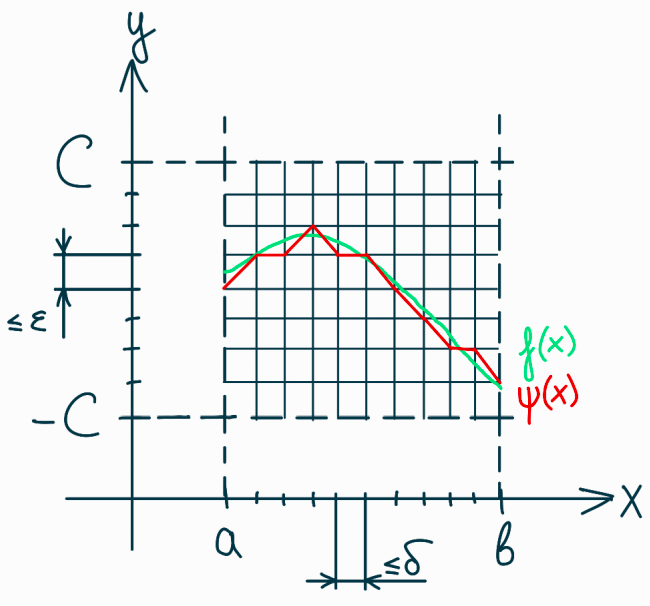
\includegraphics[width=0.5\textwidth]{images/5pic.png}
		\end{center}
		
		Более того, у нас есть равностепенная непрерывность $M$, то есть для $\eps$ найдётся $\delta > 0$. Итак, <<порежем>> прямоугольник на одинаковые части по горизонтали так, что они были меньше $\delta$, а по вертикали меньше $\eps$. У нас возникнут узлы полученной сетки. Обозначим за $\{x_k\}_{k = 1}^n$ горизонтальные координаты разрезов по возрастанию (при этом $x_1 = a$, $x_n = b$ и $|x_{k + 1} - x_k| < \delta$). Кандидат в искомую $\eps$-сеть --- это множество всех ломаных функций, которые проходят по узлам решётки, причём обязательно соседние узлы функции лежат в соседних горизонтальных разрезах (то есть, если взять соседние узлы ломаной, то эти точки соответствуют аргументам $x_k$ и $x_{k + 1}$ при некотором $k$).
		
		Теперь, рассмотрим произвольную $f \in M$. Так как $|x_{k + 1} - x_k| < \delta$, то $|fx_{k + 1} - fx_k| < \eps$. Значит, за 1 сдвиг по горизонтали $f$ двигается не более чем на 1 сдвиг по вертикали (где сдвиг --- это ширина либо высота квадратика, на которые мы поделили прямоугольник соответственно). Это позволяет выбрать ломаную функцию $\psi$ из полученного выше множества так, что $|fx_k - \psi x_k| < \frac{\eps}{2}$ (то есть просто выбирали лучший приближающий узел с каждым сдвигом). Осталось показать, что $\|f - \psi\| < \eps$, а для этого рассмотрим произвольный $x \in [a; b]$. Тогда верно, что $x \in [x_k; x_{k + 1}]$ для некоторого $k$. Осталось записать неравенство на расстояние значений:
		\begin{multline*}
			|fx - \psi x| \le |fx - fx_k| + |fx_k - \psi x_k| + |\psi x_k - \psi x| \le
			\\
			|fx - fx_k| + |fx_k - \psi x_k| + |\psi x_k - \psi x_{k + 1}|
		\end{multline*}
		Последний переход верен в силу линейности $\psi$ между $[x_k; x_{k + 1}]$. Первое слагаемое меньше $\eps$ по равностепенной непрерывности, второе меньше $\eps$ в силу построения, осталось формально разобраться с последним, но здесь мы снова можем сослаться на построение $\psi$ и получить не больше $\eps$ (формально можно написать такое: $|\psi x_k - \psi x_{k + 1}| \le |\psi x_{k + 1} - fx_{k + 1}| + |fx_{k + 1} - fx_k| + |fx_k - \psi x_k| < 2\eps$). Итого:
		\[
			|fx - \psi x| \le \eps + \frac{\eps}{2} + \eps < 3\eps
		\]
	\end{itemize}
\end{proof}

\section{Линейные нормированные пространства}

\begin{exercise}
	Пусть $E$ --- линейное нормированное пространство над $\K$, $M = [e_1, \ldots, e_n]$. Докажите, что $M$ является замкнутым множеством.
\end{exercise}